\documentclass[]{"article"}
\usepackage{polyglossia}
\usepackage{fancyhdr}
\usepackage{enumerate}
\usepackage{framed}
\usepackage{listings}
\usepackage{amsfonts}
\usepackage[usenames,dvipsnames,svgnames,table]{xcolor}
\usepackage{minted}
\usepackage{hyperref}
\usepackage{graphicx}
\usepackage{gensymb}
\graphicspath{ {./images/} }

\setmainlanguage{spanish}
\definecolor{mygray}{RGB}{248,249,250}

\newcommand{\pythonblock}{\inputminted[linenos,bgcolor=mygray,framesep=10pt,firstnumber=\value{pythonnumber}]{python3}}
\newcommand{\asw}{\textbf{R. }}
\renewcommand{\theFancyVerbLine}{\sffamily \textcolor[rgb]{0.5,0.5,1.0}{\footnotesize \oldstylenums{\arabic{FancyVerbLine}}}}

\title{Guía de ejercicios resueltos \protect\\ Algoritmos y programación}
\author{Anggelo Urso G. \\ anggelo.urso@inacapmail.cl}
\date{\today}

\pagestyle{fancy}
\fancyhf{}
\lhead{Algoritmos y programación}
\rhead{\thepage}
\lfoot{AUG /\LaTeX}

\hypersetup{
    colorlinks=true,
    linkcolor=blue,
    filecolor=magenta,      
    urlcolor=cyan,
}

\newcounter{pythonnumber}
\setcounter{pythonnumber}{1}

\begin{document}
    \thispagestyle{empty}
    \maketitle

    \section{Introducción}
    
    El siguiente documento tiene por finalidad generar una guía de ejercicios resueltos para facilitar el aprendizaje de los alumnos de la asignatura de algoritmos y programación.

    \section{Ejercicios resueltos}

    A continuación se desarrollarán una serie de ejercicios resueltos de acuerdo a distintas secciones de interés en la materia.

    \subsection{Entrada y salida de datos}
    \begin{enumerate}[{Ejercicio} 1.]
        \item Muestre por pantalla el siguiente texto: "Hola mundo".\\

        \asw Para desarrollar este ejercicio utilizaremos la función \textbf{print}, luego nuestro código quedaría como:\\

        \pythonblock{python/entradaSalida/hola_mundo.py}

        En este caso, observamos que pasamos como argumento el \textbf{string} "Hola mundo" y luego se muestra por pantalla.
        
        \item Leer un string desde teclado. \\

        \asw Para desarrollar este ejercicio utilizaremos la función \textbf{input}. Esta función lee desde el teclado los datos. \\
        
        \pythonblock{python/entradaSalida/input_vacio.py}

        Luego si queremos mejorar un poco la entrada de los datos, agregando un texto antes para indicar al usuario que es lo que pedimos, la función \textbf{input} recibe como argumento un \textbf{string}, el cual se despliega por pantalla y solicita el texto. \\

        \pythonblock{python/entradaSalida/input_con_texto.py}

        Finalmente si queremos almacenar el valor recibido por teclado en una variable para posteriormente utilizarlo, usamos:\\

        \pythonblock{python/entradaSalida/input_con_variable.py}

        \item Leer un string desde el teclado y luego mostrarlo por pantalla.\\
        
        \asw Para este ejercicio usaremos \textbf{print} e \textbf{input}, a través de la segunda capturaremos el \textbf{string} desde teclado y con la primera lo mostraremos por pantalla.\\

        \pythonblock{python/entradaSalida/print_input.py}

        Prueba tu código con la palabra \textit{Hola}. Debería mostrarte la palabra por pantalla.

        \item Leer un numero desde teclado.\label{e.num} \\
        
        \asw Primero es necesario entender que la función \textbf{input}, lo que nos retorna al flujo del programa es un string. Para poder devolver un \textbf{int} al flujo, es necesario hacer un \textit{cast} de la variable, es decir. Si queremos un entero, debemos forzar el tipo a la función input.\\

        \pythonblock{python/entradaSalida/input_comment.py}

        \textbf{Importante:} si el dato que estamos ingresando por teclado no es un entero (ej. un flotante o un string) esto nos arrojará un error. Esto debido a que estamos forzando el tipo de dato a entero si o si.

        \item Sumar dos números recibidos desde teclado y mostrar el resultado por pantalla.\\
        
        \asw Para esto usaremos la función \textbf{input} y asignación de variables. Luego sumaremos el resultado y usaremos la función \textbf{print} para mostrar el resultado por pantalla.\\

        \pythonblock{python/entradaSalida/suma_input.py}

        Prueba tu programa escribiendo 3 y 5, el resultado por pantalla debiese ser 8.

        \item Recibir dos números flotante por teclado y mostrar la suma por pantalla sin usar una variable para la suma.\\
        
        \asw Tal y como vimos en el ejercicio \ref{e.num} para determinar el tipo de dato de la función \textbf{input} debemos forzarlo. Luego nos piden mostrar por teclado sin usar una variable para la suma, esto lo podemos hacer con la función \textbf{print} pasando directamente la suma de los números.\\

        \pythonblock{python/entradaSalida/float_input.py}

        Prueba tu programa con 3 y 5, el resultado debiese ser 8.0. Otra opción, probar con 3.0 y 5.0, como resultado también debiese ser 8.0.

        \textbf{Importante:} Acá al igual que el ejercicio \ref{e.num} estamos esperando un tipo de dato flotante. Si pasamos por error un \textbf{string} nos arrojará un error. No así si pasamos un entero, dado a que un entero "cabe" en un flotante. Más específicamente, un número flotante es más general que un entero, y el conjunto de los número enteros está contenido en los flotantes.\footnote{Esto se lee, los números enteros \(\mathbb{Z}\) son un subconjunto de los números racionales (flotantes) \(\mathbb{Q}\)}

        \[\mathbb{Z} \subset \mathbb{Q} \]

        \item Recibir un nombre desde el teclado y luego mostrar un saludo personalizado a ese nombre. \\
        
        \asw Guardamos el dato recibido por teclado en una variable y luego mostramos \textit{"Hola "} junto con el nombre recibido por teclado.

        Acá tenemos dos alternativas, la primera es pasar el saludo, y separado por una coma, el nombre ingresado por teclado. La segunda es concatenar (sumar los dos \textbf{strings}) en la función \textbf{print}.\\

        \pythonblock{python/entradaSalida/saludo_nombre.py}

        Si pruebas tu programa con el nombre \textit{Pedro} debiese retornar: \textbf{Hola Pedro} dos veces con este código (una vez si solo usaste una de las dos alternativas).

        \item Pedir el nombre al usuario por teclado y luego solicitar el apellido (también por teclado), mostrando el nombre en la entrada de datos. Luego saludar a la persona.\label{e.nom-apel}\\
        
        \asw Una de las cosas bonitas que tiene la función \textbf{input} es que podemos concatenar \textbf{strings} recibidos anteriormente en otro \textbf{input}. De esta manera podemos hacer un código de las siguiente forma.\\

        \begin{listing}[H]
            \pythonblock{python/entradaSalida/saludo_nom-apel.py}
        \end{listing}

        En este caso si ingresamos como nombre \textit{Pedro} y como apellido \textit{González}, el programa nos debería mostrar: \textbf{Hola Pedro, cuál es su apellido}, seguido por: \textbf{Mucho gusto Pedro González}

        \item Resolver el ejercicio \ref{e.nom-apel} ahora con texto formateado.\label{e.formato}\\
        
        \asw Cuando nos piden texto formateado, anteponemos una \textbf{f} antes de la cadena y luego, a través de paréntesis de llave, vamos escribiendo las variables.\\

        \begin{listing}[H]
            \pythonblock{python/entradaSalida/saludo_nombre-formato.py}
        \end{listing}

        En este caso si ingresamos como nombre \textit{Pedro} y como apellido \textit{González}, el programa nos debería mostrar: \textbf{Hola Pedro, cuál es su apellido}, seguido por: \textbf{Mucho gusto Pedro González}

        A contar de ahora en adelante, si queremos un texto \textit{con formato} usaremos esta forma para representarlo (importante la \textbf{f} y la forma de escritura).

        \item Diseñe un programa que a partir del valor del lado de un cuadrado (3 metros), muestre el valor de su perímetro (en metros) y el de su área (en metros cuadrados). \\
        
        \asw Sabemos que el perímetro de un cuadrado es la suma de sus cuatro lados, o similar:

        \[perimetro = lado * 4\]

        Y que el área es calcular el cuadrado de su lado:

        \[area = lado^2\]

        Con los datos que nos entregan, el perímetro debe darnos 12 metros y el área 9 metros cuadrados. Luego un programa que calcule el perímetro, con un valor de lado dado, sería algo como esto:\\

        \pythonblock{python/entradaSalida/perimetroCuadrado.py}

        \item Diseñe un programa que, a partir del valor de la base y de la altura de un triángulo (3 y 5 metros respectivamente), muestre el valor de su área (en metros cuadrados).\\
        
        \asw Recordamos que el cálculo del área de un triangulo viene dado por:

        \[area = \frac{base * altura}{2}\]

        Luego con los datos que nos entregan el área del triángulo debiese tener un valor de 7.5 metros cuadrados. Si hacemos un programa en Python que nos haga dicho cálculo, tenemos:\\

        \pythonblock{python/entradaSalida/areaTriangulo.py}
        
        \item Calcule el área de una circunferencia, pidiendo el radio de ésta al usuario para que lo ingrese por teclado.\\
        
        \asw El cálculo del área de una circunferencia está dado por:

        \[ area = \pi * radio^2 \]

        Python nos ofrece la librería \textbf{math} para obtener desde ella distintos tipos de funciones o constantes (entre ellas el valor de \textbf{pi}). Para usarla solo basta importarla y usarla directamente.\\

        \begin{listing}[H]
            \pythonblock{python/entradaSalida/areaCirculo.py}
        \end{listing}

        Podemos probar el programa, ingresando el valor del radio en 3, lo cual nos daría como resultado: \textbf{El área de la circunferencia es: 28.274333882308138}

        \item Calcular el volumen de una esfera, solicitando al usuario el ingreso del radio de ésta por teclado.\\
        
        \asw Recordando la fórmula

        \[ volumen = \frac{4}{3} * \pi * radio^3 \]

        Luego usamos \textbf{input} para capturar el valor del radio desde el teclado y llevamos la formula a nuestro programa, e importamos la librería \textbf{math} para obtener el valor de \textbf{pi}.\\

        \pythonblock{python/entradaSalida/areaEsfera.py}
        
        Podemos probar el programa, ingresando el valor del radio en 3, lo cual nos daría como resultado: \textbf{Volumen de esfera es: 113.09733552923254}

        \item Diseña un programa que pida el valor de los tres lados de un triángulo y calcule el valor de su área y perímetro. \\
        
        \asw Si nos recordamos, el área de un triángulo en base a sus lados (a, b, c) se calcula como:

        \[ area = \sqrt{s(s-a)(s-b)(s-c)}\]

        Donde:

        \[ s = \frac{a + b + c}{2} \]

        Acá usaremos nuevamente la librería \textbf{math} para poder usar la función de raíz cuadrada (\textbf{sqrt}). Escribiendo nuestro programa en Python, obtenemos lo siguiente:

        \begin{listing}[H]
            \pythonblock{python/entradaSalida/trianguloLados.py}
        \end{listing}

        Si probamos con lados de 3, 5 y 7; el resultado debiese ser: \textbf{El área es 6.49519052838329} y \textbf{El perímetro es 15}.

        \item Diseñe un programa que calcule el área de un triángulo a partir del valor de dos de sus lados y el ángulo entre ellos (en grados), mostrando por pantalla el resultado.\\
        
        \asw Nuevamente nos vamos a matemáticas:

        \[ area = \frac{1}{2} a*b*\sin(\theta) \]

        Siendo \textbf{a} y \textbf{b} los lados y \(\theta\) el ángulo entre ellos (en grados). Un punto importante, usaremos la librería \textbf{math} para poder usar la función \textbf{sin}. Sin embargo esta función calcula el seno de un ángulo, pero este debe estar en radianes (no en grados). Sin embargo la transformación de un ángulo en grados a radianes es bastante simple, sabiendo que \(\pi = 180\), luego aplicamos regla de 3 simple y tenemos:

        \[ radianes = grados * \frac{\pi}{180} \]

        Así nuestro código nos quedaría como:

        \begin{listing}[H]
            \pythonblock{python/entradaSalida/areaTrianguloGrados.py}
        \end{listing}

        Si probamos nuestro código con \textbf{a=1}, \textbf{b=2} y \textbf{ángulo=30}, el resultado debiese ser: \textbf{El área es 0.49999999999999994} o aproximado a \textbf{0.5}

        \item Diseñe un programa que pida al usuario una cantidad de pesos, una tasa de interés anual y un número de años y calcule cuanto habrá convertido el capital inicial transcurrido esos años, si a cada año se le calcula la tasa tasa de interés (interés compuesto).\\
        
        \asw Nos vamos a nuestra fórmula de interés compuesto (con tasa de interés en porcentaje):

        \[ monto = C * (1 + \frac{i}{100})^{n} \]

        Con \textbf{C} el capital, \textbf{i} la tasa de interés anual y \textbf{n} periodo en años. Luego si llevamos esto a nuestro programa en Python tenemos:\\

        \begin{listing}[H]
            \pythonblock{python/entradaSalida/interesCompuesto.py}
        \end{listing}

        Si probamos nuestro código con: \textbf{capital=10000}, \textbf{interés=4.5} y \textbf{periodo=20}; debiésemos obtener como resultado: \textbf{El valor final en 20 años es de: 24117.14}.

        Acá debemos notar que capital y periodo son enteros, por ende forzamos el tipo de la función \textbf{input} en entero; y que el valor de interés es un número flotante, así que forzamos el tipo a flotante.
    \end{enumerate}

    \subsection{Ejercicios con tortuga}
    En los ejercicios de la siguiente sección utilizaremos el módulo \textbf{turtle} que se encuentra en Python. Cada ejercicio importará el módulo, así que presten atención a los ejemplos.

Además mencionar que utilizaremos una versión un poco diferente de lo que vimos en clases. En particular utilizaremos y definiremos la pantalla en la cual trabajaremos, así si observan el siguiente código:\\

\begin{listing}[H]
    \pythonblock{python/tortuga/tortugaBasica.py}
\end{listing}

Observamos lo siguiente:

\begin{itemize}
    \item Importamos los elementos usando \textbf{from turtle import Screen, Turtle}. Esto lo realizamos para importar solo esas funciones de la librería turtle (y no traernos todo). En caso de que necesitemos todo, el ejercicio nos dirá directamente \textbf{import turtle}.
    \item Creamos una pantalla a través de la función \textbf{Screen()} y definimos su tamaño utilizando la función \textbf{setup} (si necesitamos más grande o más chico acá vamos ajustando) de 425 píxeles de ancho y 225 píxeles de alto.
    \item En la línea \textbf{5} fijamos el tamaño de la superficie de dibujo en 400 píxeles de ancho y 200 píxeles de alto.
    \item A través de la función de la línea \textbf{7} controlamos que la pantalla de la tortuga se cierre una vez que demos clic sobre la interfaz
\end{itemize}

Entendiendo eso como esencial comenzamos con los ejercicios resueltos\footnote{Es recomendable comenzar a leer \href{https://docs.python.org/3/library/turtle.html}{documentación del módulo de turtle}}.

\begin{enumerate}[{Ejercicio} 1.]
    \item Diseñe un programa que dibuje un cuadrado por la pantalla de lado 100.\\
    
    \asw Para esto utilizaremos la función \textbf{fd} para mover nuestra tortuga 100 pasos hacia adelante y \textbf{rt} para girar a la derecha\footnote{\textbf{rt} es el nombre corto de \textbf{right}, al igual que \textbf{fd} es el nombre corto de \textbf{forward} o \textbf{lt} es de \textbf{left}}.\\

    \begin{listing}[H]
        \pythonblock{python/tortuga/cuadrado-turtle.py}
    \end{listing}

    El resultado debiese entregar esta figura\\

    \begin{figure}[H]
        \centering
        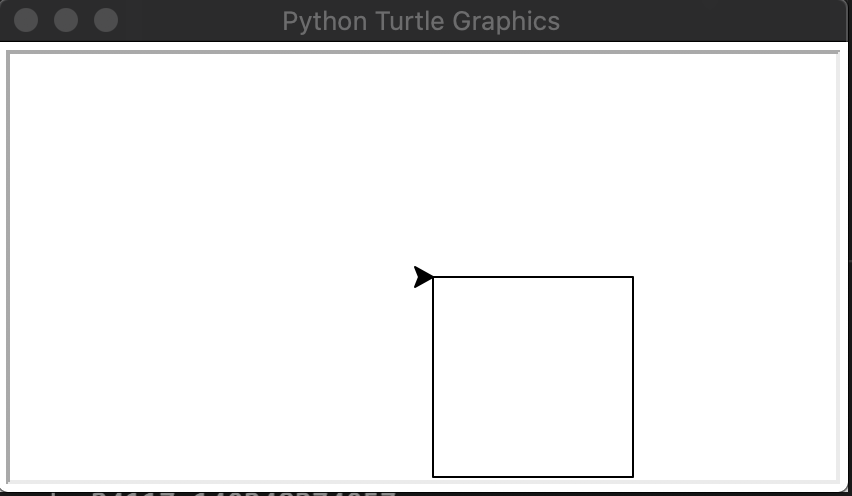
\includegraphics[scale=0.4]{cuadrado}
    \end{figure}

    \item Diseñe un programa que dibuje en la pantalla un triángulo equilátero de lado 100.\\
    
    \asw Para que sea un triángulo equilátero, todos sus lados miden lo mismo y los ángulos interiores son de \(60\degree\). Para esto usamos la función \textbf{lt} para hacer el triángulo hacia arriba. Además consideramos pasar \(120\) como valor a la función \textbf{lt} (diferencia entre 180 - 60). Así el código nos queda como:\\

    \begin{listing}[H]
        \pythonblock{python/tortuga/triangulo-turtle.py}
    \end{listing}

    Luego deberíamos ver por pantalla:

    \begin{figure}[H]
        \centering
        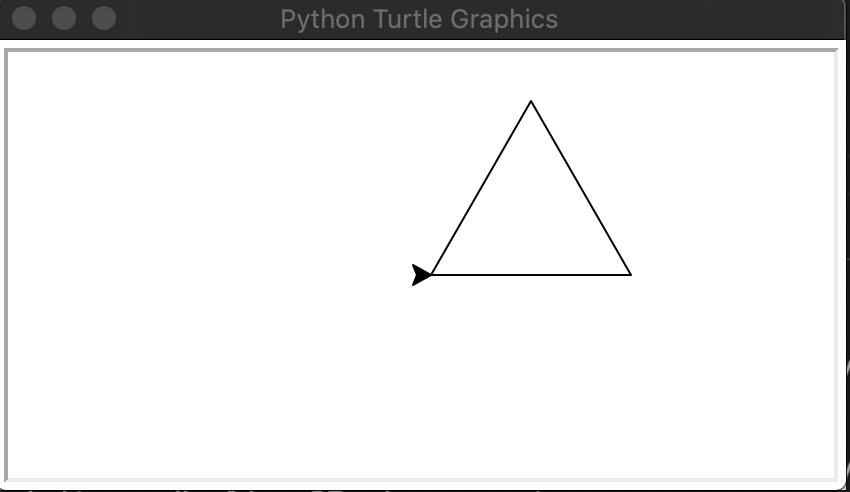
\includegraphics[scale=0.4]{triangulo}
    \end{figure}

    \item Diseñe un programa que dibuje un cuadrado cuyos lados midan 200 pasos y otro cuadrado cuyos lados midan 100 centrado al interior del cuadrado más grande.
    
    \asw Para esto usaremos \textbf{up} y \textbf{down} que levantan el pincel y lo bajan respectivamente. Con esto podemos mover libremente la tortuga sin pintar sobre el lienzo.

    Para posicionar a la tortuga dentro del cuadrado grande, levantaremos el pincel y nos moveremos 50 pasos hacia el frente y 50 pasos hacia abajo. Una vez en esa posición dibujaremos el segundo cuadrado y nos quedará centrado. Así el código quedaría:\\

    \begin{listing}[H]
        \pythonblock{python/tortuga/inception-cuadrado-turtle.py}
    \end{listing}

    Y obtendremos como resultado la siguiente figura:\\

    \begin{figure}[H]
        \centering
        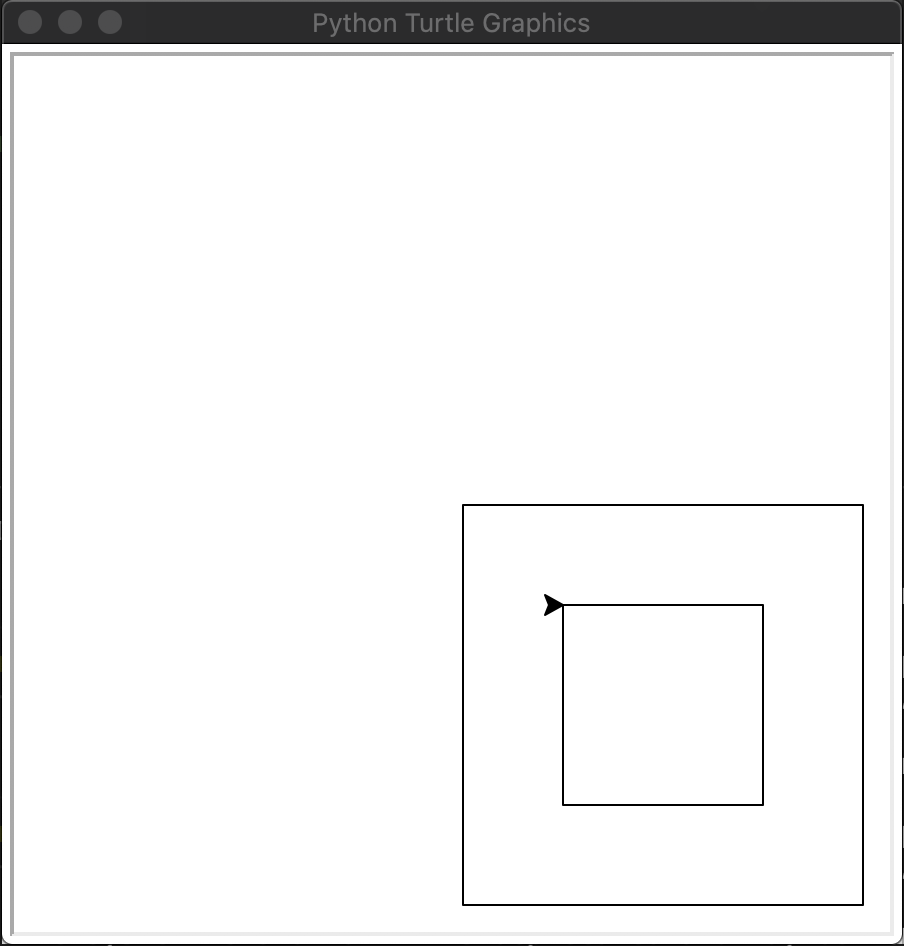
\includegraphics[scale=0.4]{cuadrado-inception}
    \end{figure}

    \item Diseñar un programa que permita visualizar un gráfico de torta a través de la aplicación \textbf{turtle} en donde exista la siguiente distribución de porcentajes: suspensos 10\%, 20\% de aprobados, un 40\% de notables y un 30\% de sobresalientes.\\
    
    \asw Para desarrollar este programa, lo realizaremos paso a paso. Lo primero que se realizará es el círculo de nuestro gráfico de torta. Para esto definiremos una circunferencia de radio 300. Moveremos el pincel desde la posición \textit{(0,0)} a la posición \textit{(0,-300)} para dejar un gráfico centrado en la ventana.\\

    \begin{listing}[H]
        \pythonblock{python/tortuga/pastel-1.py}
    \end{listing}

    Con esto tendremos una imagen de este tipo:\\

    \begin{figure}[H]
        \centering
        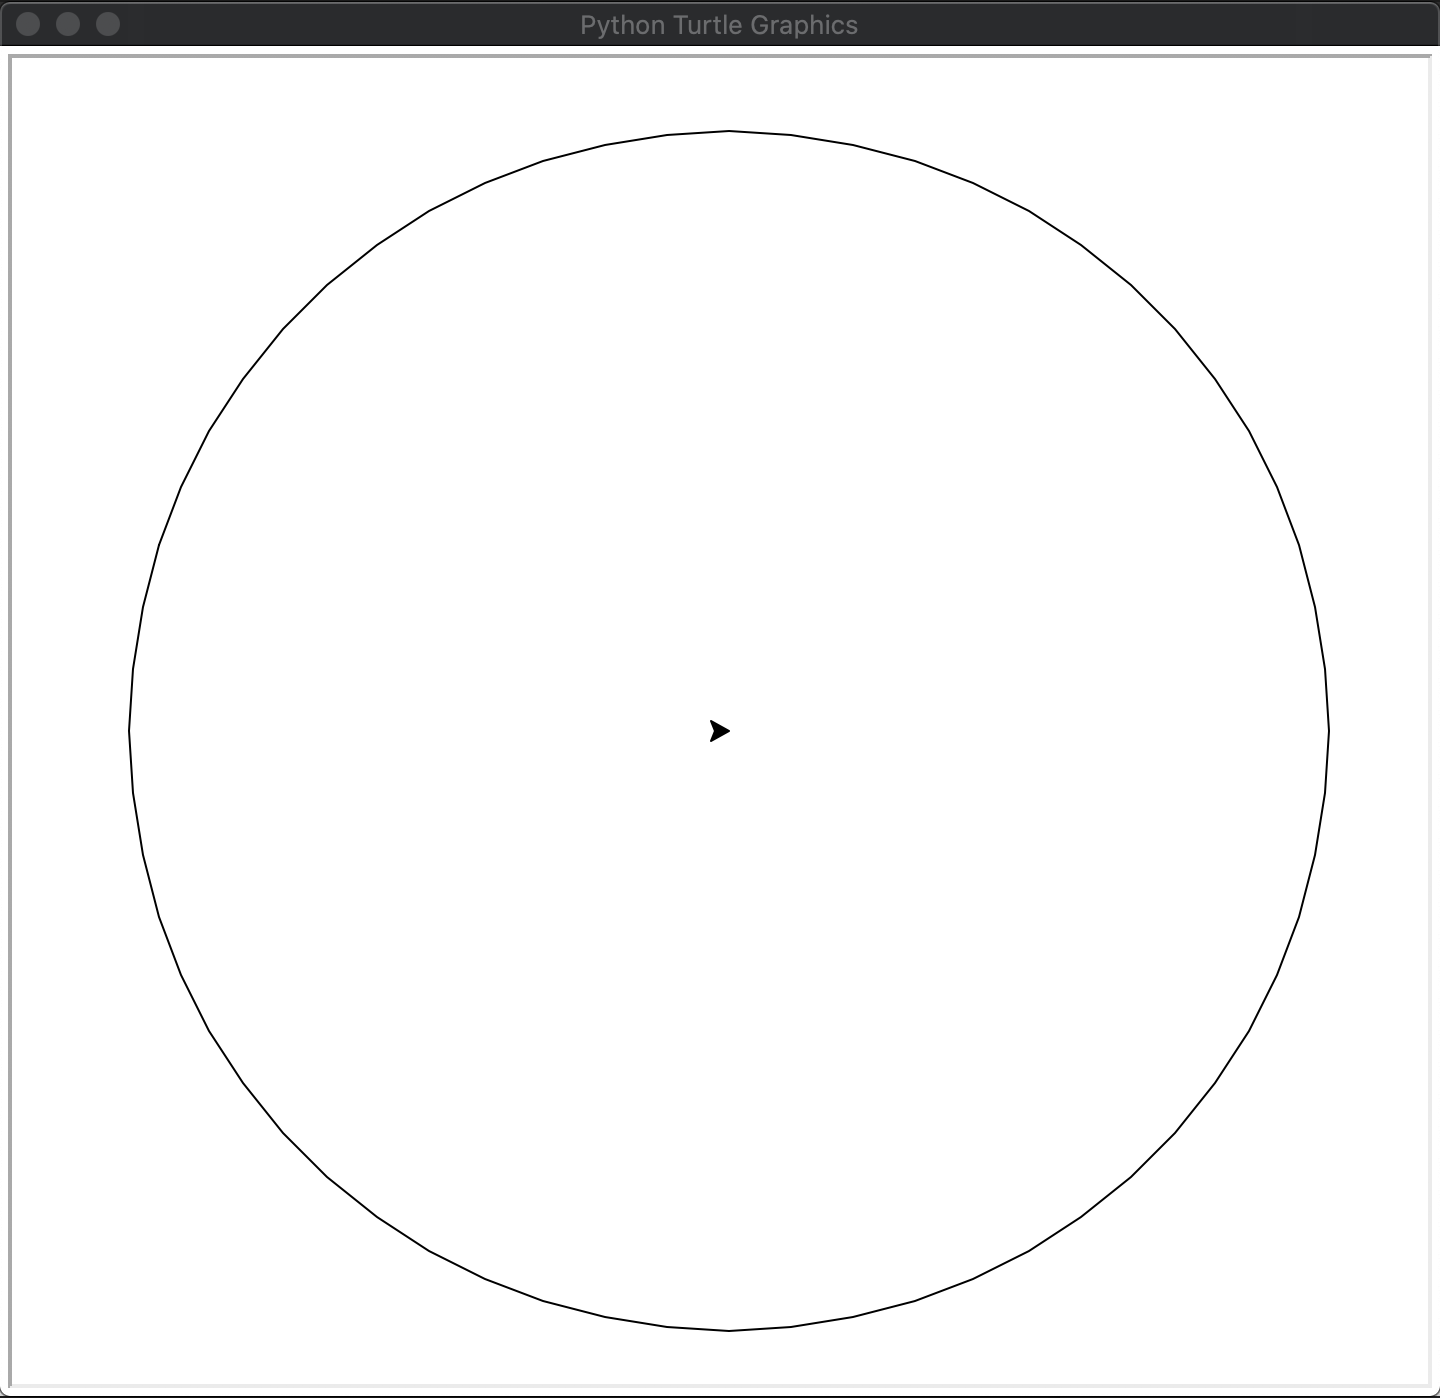
\includegraphics[scale=0.4]{circulo-1}
    \end{figure}

    Con la función \textbf{tortuga.home()} movemos al pincel a la posición inicial \textit{(0,0)}. Al levantar y bajar el pincel a conveniencia podemos graficar el círculo sin graficar todos los movimientos de éste al moverlo a los puntos de inicio del dibujo de la circunferencia.

    Guardamos las calificaciones en variables y agregamos comentarios para mayor claridad de nuestro código, así el código nos quedaría de la siguiente forma:\\

    \begin{listing}[H]
        \pythonblock{python/tortuga/pastel-2.py}
    \end{listing}

    Luego si queremos dibujar las líneas divisoras de las calificaciones, tendremos que calcular los ángulos necesarios de cada una de las calificaciones. Para esto usaremos la fórmula:

    \[ angulo_{calificacion} = \frac{360 * tipo_{nota}}{100} \]

    Así haciendo el lineamiento por cada uno de los porcentajes de notas, tenemos el siguiente código:\\

    \begin{listing}[H]
        \pythonblock{python/tortuga/pastel-3.py}
    \end{listing}

    \setcounter{pythonnumber}{40}

    \begin{listing}[H]
        \pythonblock{python/tortuga/pastel-31.py}
    \end{listing}

    Acá observamos también la función \textbf{write} que nos permite escribir un texto en el gráfico. Así nos quedaría el gráfico de la siguiente manera:\\

    \begin{figure}[H]
        \centering
        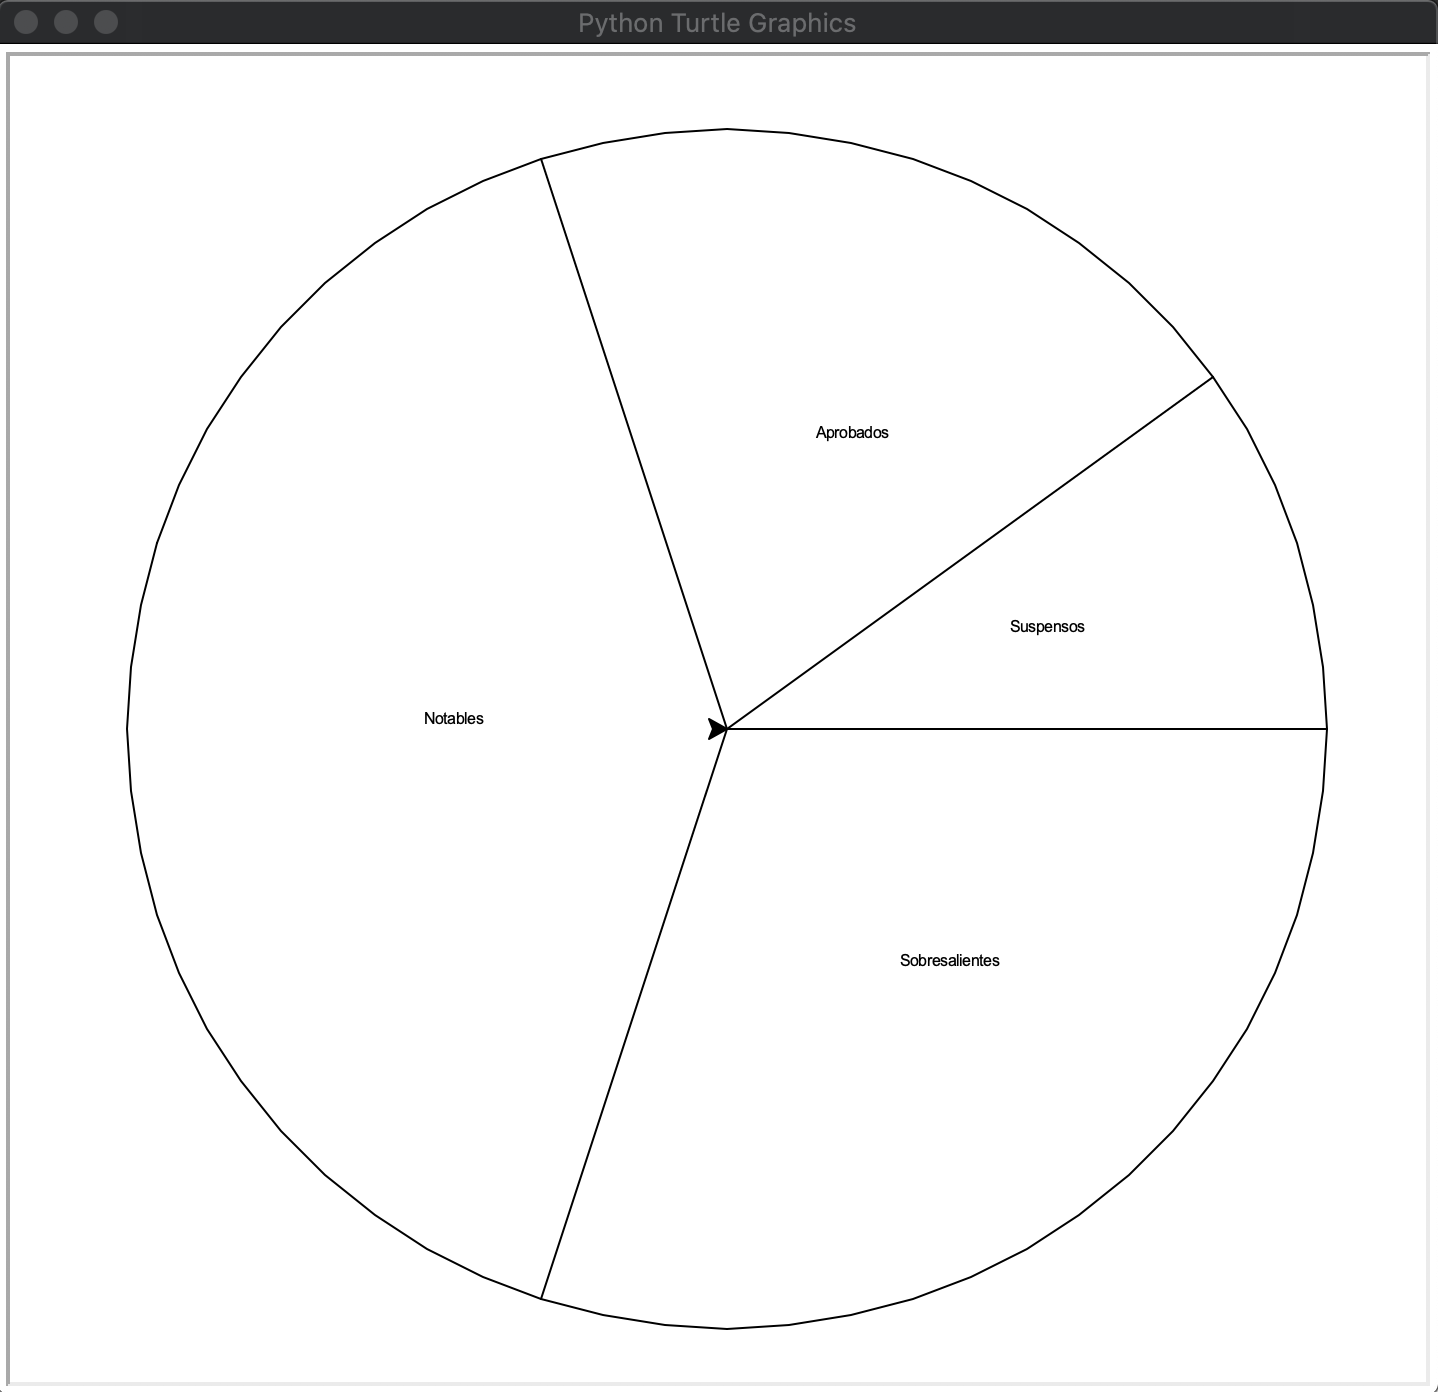
\includegraphics[scale=0.4]{circulo-3}
    \end{figure}

    \setcounter{pythonnumber}{1}

\end{enumerate}

    \subsection{Sentecias de control}
    A continuación realizaremos ejercicios con las sentencias de control de flujo \textbf{IF}, \textbf{ELSE}, \textbf{ELIF}. Iremos construyendo ejercicios en orden de relevancia y avanzando desde ejercicios simples a más complejos.

\begin{enumerate}[{Ejercicio} 1.]
    \item Diseñe un programa que reciba la edad de una persona y que muestre por pantalla si es mayor de edad.\label{e.edad}\\
    
    \asw Usamos la sentencia \textbf{IF} para evaluar la condición: \( edad > 18 \). Si esta es verdad (\textbf{True}) entonces nos va a mostrar el mensaje, en caso contrario, no va a mostrar nada. El código quedaría como:\\

    \begin{listing}[H]
        \pythonblock{python/sentenciasControl/edad.py}
    \end{listing}

    Si probamos con \(edad = 21\), el programa debería mostrar: \textbf{Es mayor de edad}.

    \item Rediseñe el programa del ejercicio \ref{e.edad} para incluir un mensaje que indique que la persona no es mayor de edad.\\
    
    \asw Para esto reformularemos el programa anterior y usaremos la sentencia \textbf{ELSE}. Esta sentencia se ejecutará solo cuando la condición \( edad > 18 \) sea falsa (\textbf{False}).\\

    \begin{listing}[H]
        \pythonblock{python/sentenciasControl/edad-else.py}
    \end{listing}

    Si probamos con \(edad = 21\), el programa debería mostrar: \textbf{Es mayor de edad}.

    Si probamos con \(edad = 15\), el programa debería mostrar: \textbf{Es menor de edad}.

    \item Solicitar la edad de dos personas por teclado e indicar que persona es mayor, menor o si tienen la misma edad.\\
    
    \asw Para esto usaremos la sentencia \textbf{IF} y la sentencia \textbf{ELSE} para validar quien es mayor. Para esto compararemos \(edad_{p1} > edad_{p2} \), si es verdad entonces la persona 1 es mayor que la persona 2, pero si es falsa se nos abren dos posibilidades:\\

    \begin{enumerate}
        \item Que ambas personas tengan la misma edad
        \item Que la persona 2 es mayor que la persona 1
    \end{enumerate}

    Con esto en mente, tenemos que en la sentencia \textbf{ELSE} considerar ambos escenarios. Así podemos considerar esto como otra sentencia de control de flujo.\\

    \begin{listing}[H]
        \pythonblock{python/sentenciasControl/edad-personas.py}
    \end{listing}

    Una mejora de código que podemos proponer en el código anterior, es la utilización de la sentencia \textbf{ELIF}, así nuestro código quedaría como:

    \begin{listing}[H]
        \pythonblock{python/sentenciasControl/edad-persona-elif.py}
    \end{listing}

    Ahora podemos probar con los siguientes valores:

    \begin{enumerate}
        \item Edad1 = 20, edad2 = 15; el resultado debe ser: \textbf{La persona 1 es mayor}
        \item Edad1 = 15, edad2 = 21; el resultado debe ser: \textbf{La persona 2 es mayor}
        \item Edad1 = 15, edad2 = 15; el resultado debe ser: \textbf{Las personas tienen la misma edad}
    \end{enumerate}

    \item Diseñe un programa que determine si un número ingresado por el usuario es par o impar y muestre un mensaje según corresponda. \\
    
    \asw Para esto utilizaremos la operación módulo (\%). Esta operación nos entrega el resto de una división. Si esta es exacta el resultado de la operación es 0, si la división no es exacta, nos entregará el resto de la división. Para determinar si el número es par o no, simplemente tenemos que calcular la operación módulo de 2 con el número. Si este es par, el resultado será cero, en caso contrario entregará 1. Así nuestro código quedará como:\\

    \begin{listing}[H]
        \pythonblock{python/sentenciasControl/esPar.py}
    \end{listing}

    Así, si ingresamos el número \textbf{8}, el programa nos entregará: \textbf{El número 8 es par}; si ahora probamos con el número \textbf{15}, el programa nos entregará: \textbf{El número 15 es impar}.

    \item Diseñe un programa usando el módulo \textbf{turtle}, que en base a 3 opciones, presentadas en un menú, dibuje: un cuadrado, un triángulo o un círculo.\\
    
    \asw Si definimos que nuestras opciones son:

    \begin{enumerate}
        \item cuadrado
        \item triángulo
        \item circulo
    \end{enumerate}

    Tenemos que crear el menú y obtener la opción escogida por el usuario desde el teclado, y en base a esa opción dibujar. En este caso podríamos observar como quedaría el código:\\

    \begin{listing}[H]
        \pythonblock{python/sentenciasControl/tortuga-menu.py}
    \end{listing}

    Si observamos, capturamos la opción del usuario y según la opción escogida mostramos una figura u otra. Si mejoramos un poco más el código usando \textbf{string} multilinea (ahorrándonos los 4 \textbf{print}) y por otro lado usamos la sentencia \textbf{ELIF} por el sangrado, nos queda un código un poco más limpio:\\

    \begin{listing}[H]
        \pythonblock{python/sentenciasControl/tortuga-menu-revisited.py}
    \end{listing}

    \item Diseñe un programa que permita calcular el valor de \textbf{x} de la siguiente ecuación. Los valores de \(a\) y \(b\) serán ingresados por teclado.
    
    \[ ax + b = 0 \]

    \asw Para resolver esta ecuación, debemos despejar la \(x\). Esto lo hacemos moviendo los términos hacia el otro lado de la ecuación, quedándonos de la siguiente manera:\\

    \[ x = \frac{-b}{a} \]

    \begin{listing}[H]
        \pythonblock{python/sentenciasControl/ec-primer-1.py}
    \end{listing}

    Luego, acá se nos presenta un problema. Si el usuario ingresa un valor de \(a = 0\), esta ecuación nos entrega un error de división por 0. Esto se produce dado a que la ecuación no tiene valores posibles para resolverse.

    Otro escenario que es posible apreciar acá es cuando el usuario ingresa un valor de \(a=0\) y \(b=0\). En ese caso, la ecuación tiene infinitas soluciones. Sin embargo esos dos casos no los estamos graficando correctamente en nuestro código, para eso tenemos que considerar ambas restricciones y colocar los respectivos mensajes, quedando nuestro código de la siguiente manera:\\

    \begin{listing}[H]
        \pythonblock{python/sentenciasControl/ec-primer-2.py}
    \end{listing}

    \item Diseñe un programa que permita calcular los valores que toma \(x\) en una ecuación de segundo grado, en donde los valores de \(a\), \(b\) y \(c\) son ingresados por el usuario por teclado. Recordar que para obtener los valores de x, se debe resolver la siguiente ecuación:
    
    \[ x = \frac{-b \pm \sqrt{b^2 - 4*a*c}}{2*a}\]

    \asw Para este ejercicio lo iremos desarrollando por partes. 
    
    Lo primero que debemos validar, son las entradas de los valores de \(a\), \(b\) y \(c\).

    Si observamos la fórmula anterior, observamos que el primer problema que podemos tener es que el usuario ingrese un valor de \(a=0\). Con esto el cálculo de los valores de \(x\) se indefine, dado a que me quedaría una división por 0. Por otro lado, si observamos como planteamos una ecuación de segundo grado:

    \[ ax^2 + bx + c = 0 \]

    Por ende, si \(a=0\), entonces se nos transforma a una ecuación de primer grado, quedando como:
    
    \[ bx + c = 0 \]
    
    Despejando x, nos queda:

    \[ x = \frac{-c}{b} \]
    
    Para este escenario podemos tener una primera versión de código de la siguiente manera:\\

    \begin{listing}[H]
        \pythonblock{python/sentenciasControl/ec-seg-1.py}
    \end{listing}

    Bien, salvamos el primer problema (pero no el único). ¿Qué pasa ahora si el usuario ingresa \(a=0\) y \(b=0\)?. Nuevamente estamos frente a un potencial error de división por 0. Para esto añadiremos más sentencias de control, tal y como hicimos cuando resolvimos la ecuación de primer grado.\\

    \begin{listing}[H]
        \pythonblock{python/sentenciasControl/ec-seg-2.py}
    \end{listing}
    
    Como los niveles de indentación (sangrado) nos van quedando incómodos, usamos la sentencia \textbf{ELIF} para agrupar mejor, quedando un código como:\\

    \begin{listing}[H]
        \pythonblock{python/sentenciasControl/ec-seg-3.py}
    \end{listing}

    Ok, hasta este punto podemos calcular los valores de \(x\) reales, pero seguimos teniendo un problema, ¿qué pasa si el discriminante es negativo?.

    Determinamos al discriminante de la ecuación de segundo grado al cálculo que realizamos dentro de la raíz cuadrada:

    \[ \Delta = b^2 - 4 * a * c \]

    El problema es que si este valor es negativo la ecuación no tendrá soluciones reales. Por otro lado, la librería \textbf{math}, y en particular la función \textbf{sqrt} no permite resolver raíces cuadradas negativas, entonces debemos realizar esta validación.\\

    \begin{listing}[H]
        \pythonblock{python/sentenciasControl/ec-seg-4.py}
    \end{listing}

    Hasta este punto, tenemos nuestra ecuación validada y podemos resolver los valores de \(x\) siempre que estos sean reales, en caso contrario nos mostrará por pantalla: \textbf{La ecuación no tiene soluciones reales}.

    Pero nuevamente dejamos por fuera un escenario más. Que sucede si me interesa saber las soluciones \textit{complejas} de la ecuación, al igual que las soluciones reales, ¿cómo resolvemos eso?.

    Para resolver el problema, hay un truco sumamente simple y útil que podemos usar:

    \[ \sqrt{a * b} = \sqrt{a} * \sqrt{b} \]

    Luego, si tenemos por ejemplo:

    \[ \sqrt{-5} = \sqrt{5} * \sqrt{-1} \]

    Y por definición de números complejos:

    \[ j = \sqrt{-1} \]

    Luego:

    \[ \sqrt{-5} = \sqrt{5} * j \]

    Por ende si el discriminante es negativo (señalizado acá como \(\Delta\)), podemos hacer lo siguiente:

    \[ \sqrt{-\Delta} = \sqrt{\Delta} * j \]

    Quedándonos la ecuación como:

    \[ x = \frac{-b \pm \sqrt{\Delta}j}{2*a} = \frac{-b}{2*a} \pm \frac{\sqrt{\Delta}}{2*a}j \]

    Con esto claro, colocamos la última modificación de código:\\

    \begin{listing}[H]
        \pythonblock{python/sentenciasControl/ec-seg-5.py}
    \end{listing}

    Por simple comodidad de código, hemos definido la variable \(det = 2 * a\) para mayor claridad del código.

    En la línea 15, lo que hacemos es invertir el valor del discriminante (agregando el menos delante) y así poder calcular la raíz de forma segura. Luego usando la función \textbf{complex} creamos el número complejo. 

    El primer parámetro de esa función es la parte real del número complejo, y el segundo parámetro es la parte compleja.

\end{enumerate}

\end{document}